\documentclass[journal,12pt,twocolumn]{IEEEtran}

\usepackage{enumitem}
\usepackage{amsmath}
\usepackage{amssymb}
\usepackage{gensymb}
\usepackage{graphicx}
\usepackage{txfonts}         
\usepackage{listings}
\usepackage{lstautogobble}
\usepackage{mathtools}

\newcommand{\solution}{\noindent \textbf{Solution: }}
\providecommand{\pr}[1]{\ensuremath{\Pr\left(#1\right)}}
\providecommand{\brak}[1]{\ensuremath{\left(#1\right)}}
\providecommand{\cbrak}[1]{\ensuremath{\left\{#1\right\}}}
\providecommand{\sbrak}[1]{\ensuremath{\left[#1\right]}}
\providecommand{\mean}[1]{E\left[ #1 \right]}
\providecommand{\var}[1]{\mathrm{Var}\left[ #1 \right]}
\providecommand{\der}[1]{\mathrm{d} #1}
\providecommand{\gauss}[2]{\mathcal{N}\ensuremath{\left(#1,#2\right)}}

\let\StandardTheFigure\thefigure
\let\vec\mathbf

\numberwithin{equation}{section}
\renewcommand{\thefigure}{\theenumi}
\renewcommand\thesection{\arabic{section}}

\newcommand{\myvec}[1]{\ensuremath{\begin{pmatrix}#1\end{pmatrix}}}
\newcommand{\mydet}[1]{\ensuremath{\begin{vmatrix}#1\end{vmatrix}}}

\lstset {
	frame=single, 
	breaklines=true,
	columns=fullflexible,
	autogobble=true
}             
                               
\title{Random Numbers \\ \Large AI1110: Probability and Random Variables \\ \large Indian Institute of Technology Hyderabad}
\author{Dhatri Reddy \\ \normalsize AI21BTECH11030 \\ \vspace*{20pt} \normalsize  8 July 2022}


\begin{document}

	\maketitle
	
	\section{Uniform Random Numbers}
	Let $U$ be a uniform random variable between 0 and 1.
	\begin{enumerate}[label=\thesection.\arabic*,ref=\thesection.\theenumi]
	\item Generate $10^6$ samples of $U$ using a C program and save into a file called uni.dat

	\solution Download the C source code by executing the following commands
	\begin{lstlisting}
		wget https://github.com/Dhatrireddyy/Random-numbers/blob/main/exrand.c
		wget https://github.com/Dhatrireddyy/Random-numbers/blob/main/coeffs.h
	\end{lstlisting}
	Compile and run the C program by executing the following
	\begin{lstlisting}
		cc -lm 1.1.c
		./a.out
	\end{lstlisting}
	
	\item Load the uni.dat file into Python and plot the empirical CDF of $U$ using the samples in uni.dat. The CDF is defined as
	\begin{align}
		F_{U}(x) = \pr{U \le x}
	\end{align}

	\solution  Download the following Python code that plots Fig. \ref{Figure_1}
	\begin{lstlisting}
		wget https://github.com/Dhatrireddyy/Random-numbers/blob/main/cdf_plot.py
	\end{lstlisting}
	Run the code by executing
	\begin{lstlisting}
		python cdf_plot.py
	\end{lstlisting}
	\begin{figure}
		\centering
		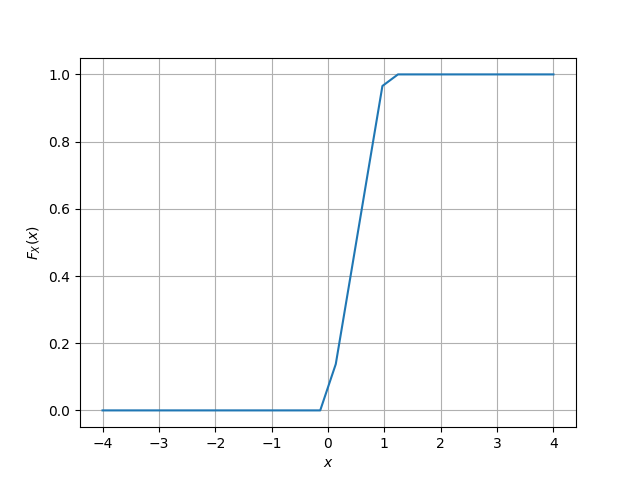
\includegraphics[width=\columnwidth]{figs/Figure_1.png}
		\caption{The CDF of $U$}
		\label{Figure_1.png}
	\end{figure}
	
	\item Find a  theoretical expression for $F_{U}(x)$
	
	\solution The PDF of $U$ is given by
	\begin{align}
		p_{U}(x) = 
		\begin{cases}
			1 & x \in [0, 1] \\
			0 & \text{otherwise}
		\end{cases}
	\end{align}
	
	The CDF of $U$ is given by
	\begin{align}
		F_{U}(x) = \pr{U \le x} = \int_{-\infty}^x p_{U}(x) ~\mathrm{d}x
	\end{align}
	
	If $x<0$,
	\begin{align}
		\int_{-\infty}^x p_{U}(x) ~\mathrm{d}x = \int_{-\infty}^x 0 ~\mathrm{d}x = 0
	\end{align}
	
	If $c$,
	\begin{align}
		\int_{-\infty}^x p_{U}(x) ~\mathrm{d}x &= \int_{-\infty}^0 0 ~\mathrm{d}x + \int_0^x 1 ~\mathrm{d}x \\
		&= 0 + x \\
		&= x
	\end{align}
	
	If $x>1$,
	\begin{multline}
		\int_{-\infty}^x p_{U}(x) ~\mathrm{d}x \\= \int_{-\infty}^0 0 ~\mathrm{d}x + \int_0^1 1 ~\mathrm{d}x +  \int_1^x 0 ~\mathrm{d}x 
	\end{multline}
	\begin{align}
		\int_{-\infty}^x p_{U}(x) ~\mathrm{d}x &= 0 + 1 + 0 \\
		&= 1
	\end{align}
	
	Therefore, we obtain the CDF of $U$ as
	\begin{align}
		F_{U}(x) = 
		\begin{cases}
			0 & x < 0 \\
			x & 0 \le x \le 1 \\
			1 & x > 1
		\end{cases}
	\end{align}
	
	\item The mean of $U$ is defined as
	\begin{align}
		\mean{U} = \frac{1}{N}\sum_{i=1}^{N}U_i
	\end{align}
	and its variance as
	\begin{align}
		\var{U} = \mean{U- \mean{U}}^2 
	\end{align}
	Write a C program to  find the mean and variance of $U$
	
	\solution Download the C source code by executing the following commands
	\begin{lstlisting}
		wget https://github.com/Dhatrireddyy/Random-numbers/blob/main/1.4.c
		wget https://github.com/Dhatrireddyy/Random-numbers/blob/main/header.h
	\end{lstlisting}
	Compile and run the C program by executing the following
	\begin{lstlisting}
		cc -lm 1.4.c
		./a.out
	\end{lstlisting}
	The output of the code is
	\begin{align}
		\mu_{\text{emp}} &= 0.500007 \\
		\mu_{\text{the}} &= 0.500000 \\
		\sigma_{\text{emp}}^2 &= 0.083301 \\
		\sigma_{\text{the}}^2 &= 0.083333
	\end{align}
	
	\item Verify your result theoretically given that
	\begin{align}
		\mean{U^k} = \int_{-\infty}^{\infty}x^k \mathrm{d}F_{U}(x)
	\end{align}
		
	\solution The mean of $U$ is given by
	\begin{align}
		\mean{U} = \int_{-\infty}^{\infty}x ~\mathrm{d}F_{U}(x) 
	\end{align}
	On differentiating the CDF of $U$, we get
	\begin{align}
		\mathrm{d}F_{U}(x) = 
		\begin{cases}
			0 & x < 0 \\
			\mathrm{d}x & 0 \le x \le 1 \\
			0 & x > 1
		\end{cases}
	\end{align}
	\begin{align}
		\therefore \mean{U} = \int_{0}^{1}x ~\mathrm{d}x = \frac12 = 0.5
	\end{align}
	
	Similarly,
	\begin{align}
		\therefore \mean{U^2} = \int_{0}^{1}x^2 ~\mathrm{d}x = \frac13
	\end{align}
	Now, the variance of $U$ is given by
	\begin{align}
		&\var{U} \\
		&= \mean{U- \mean{U}}^2 \\
		&= \mean{U^2 - 2U\mean{U} + (\mean{U})^2}
	\end{align}
	By linearity of expectation, we have
	\begin{align}
		&\mean{U^2} + \mean{-2U\mean{U}} + \mean{(\mean{U})^2} \\
		&= \mean{U^2} -2\mean{U}\mean{U} + (\mean{U})^2 \\
		&= \mean{U^2} - (\mean{U})^2 \\
		&= \frac13 - \brak{\frac12}^2 \\
		&= \frac{1}{12} \approx 0.083333
	\end{align}
	
	\end{enumerate}
	
	\section{Central Limit Theorem}

	\begin{enumerate}[label=\thesection.\arabic*,ref=\thesection.\theenumi]
	\item Generate $10^6$ samples of the random variable
	\begin{align}
		X = \sum_{i=1}^{12}U_i -6
	\end{align}

	using a C program, where $U_i, i = 1,2,\dots, 12$ are  a set of independent uniform random variables between 0 and 1 and save in a file called gau.dat
	
	\solution Download the C source code by executing the following commands
	\begin{lstlisting}
		wget https://github.com/Dhatrireddyy/Random-numbers/blob/main/2.1.c
		wget https://github.com/Dhatrireddyy/Random-numbers/blob/main/header.h
	\end{lstlisting}
	Compile and run the C program by executing the following
	\begin{lstlisting}
		cc -lm 2.1.c
		./a.out
	\end{lstlisting}
		
	\item Load gau.dat in Python and plot the empirical CDF of $X$ using the samples in gau.dat. What properties does a CDF have?

	\solution Download the following Python code that plots Fig. \ref{Figure_2}
	\begin{lstlisting}
		wget https://github.com/Dhatrireddyy/Random-numbers/blob/main/2.2.py
	\end{lstlisting}
	Run the code by executing
	\begin{lstlisting}
		python 2.2.py
	\end{lstlisting}
	\begin{figure}
		\centering
		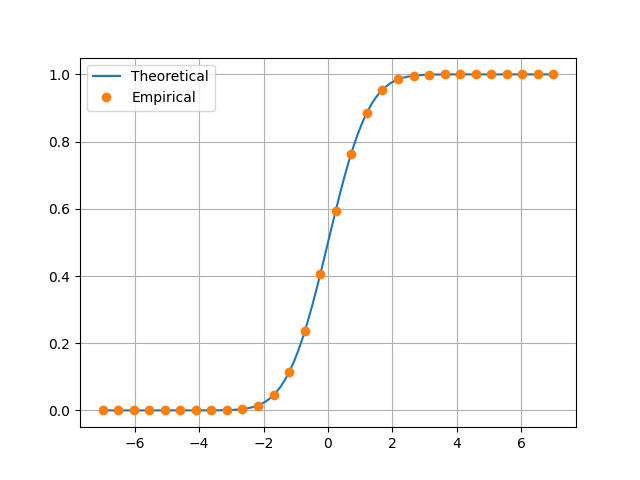
\includegraphics[width=\columnwidth]{figs/Figure_3.png}
		\caption{The CDF of $X$}
		\label{Figure_3}
	\end{figure}
	
	Every CDF is monotone increasing and right-continuous. Furthermore,
	\begin{align}
		\lim_{x \to -\infty} F_{X}(x) = 0 \qquad \lim_{x \to \infty} F_{X}(x) = 1
	\end{align}
	Thus, every CDF is bounded between $0$ and $1$ and hence, convergent.
	
	In this case, the CDF is also left-continuous. Therefore, $X$ is a continuous random variable.
	
	\item Load gau.dat in Python and plot the empirical PDF of $X$ using the samples in gau.dat. The PDF of $X$ is defined as
	\begin{align}
		p_{X}(x) = \frac{\der{}}{\der{x}}F_{X}(x)
	\end{align}
	What properties does the PDF have?
	
	\solution Download the following Python code that plots Fig. \ref{Figure_2}
	\begin{lstlisting}
		wget https://github.com/Dhatrireddyy/Random-numbers/blob/main/pdf_plot.py
	\end{lstlisting}
	Run the code by executing
	\begin{lstlisting}
		python pdf_plot.py
	\end{lstlisting}
	\begin{figure}
		\centering
		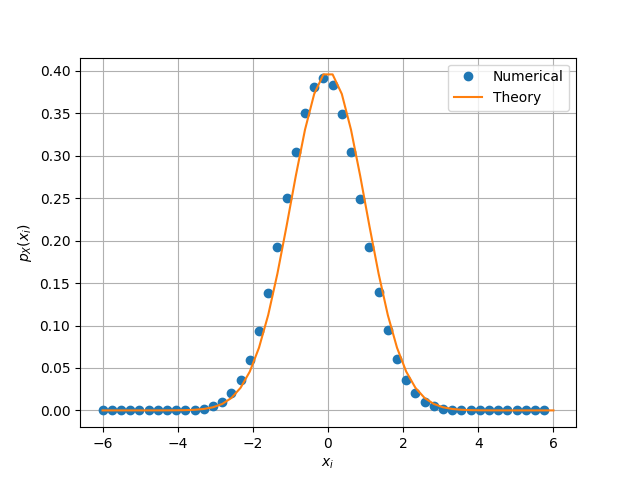
\includegraphics[width=\columnwidth]{figs/Figure_2.png}
		\caption{The PDF of $X$}
		\label{Figure_2}
	\end{figure}
	
	Every PDF is bounded between $0$ and $1$ and
	\begin{align}
		\int_{-\infty}^{\infty} p_{X}(x) ~\mathrm{d}x = 1
	\end{align}
	
	In this case, the PDF is symmetric about $x = 0$
	
	\item Find the mean and variance of $X$ by writing a C program
	
	\solution Download the C source code by executing the following commands
	\begin{lstlisting}
		wget https://github.com/Dhatrireddyy/Random-numbers/blob/main/header.h
		wget 
	\end{lstlisting}
	Compile and run the C program by executing the following
	\begin{lstlisting}
		cc -lm 2.4.c
		./a.out
	\end{lstlisting}
	The output of the code is
	\begin{align}
		\mu_{\text{emp}} &= 0.000294 \\
		\mu_{\text{the}} &= 0.000000 \\
		\sigma_{\text{emp}}^2 &= 0.999560 \\
		\sigma_{\text{the}}^2 &= 1.000000
	\end{align}	
	
	\item Given that 
	\begin{align}
		p_{X}(x) = \frac{1}{\sqrt{2\pi}}\exp\brak{-\frac{x^2}{2}}, -\infty < x < \infty,
	\end{align}
	repeat the above exercise theoretically
	
	\solution The mean of $X$ is given by
	\begin{align}
		\mean{X} &= \int_{-\infty}^{\infty} x p_{X}(x) \mathrm{d}x \\
		&= \int_{-\infty}^{\infty} \frac{x}{\sqrt{2\pi}}\exp\brak{-\frac{x^2}{2}} \mathrm{d}x 
	\end{align}
	Now, let
	\begin{align} 
		g(x) &= \dfrac{x}{\sqrt{2\pi}}\exp\brak{-\frac{x^2}{2}} \\
		\implies g(-x) &= \dfrac{-x}{\sqrt{2\pi}}\exp\brak{-\frac{(-x)^2}{2}} \\
		&= - \dfrac{x}{\sqrt{2\pi}}\exp\brak{-\frac{x^2}{2}} \\
		&= - g(x)
	\end{align}
	Thus, $g(x)$ is an odd function 
	\begin{align}
		\therefore \mean{X} &= \int_{-\infty}^{\infty} g(x) \mathrm{d}x = 0
	\end{align}
	
	Now, 
	\begin{align}
		\mean{X^2} &= \int_{-\infty}^{\infty} x^2 p_{X}(x) \mathrm{d}x \\
		&= \int_{-\infty}^{\infty} \frac{x^2}{\sqrt{2\pi}}\exp\brak{-\frac{x^2}{2}} \mathrm{d}x \\
		&= 2 \int_{0}^{\infty} \frac{x^2}{\sqrt{2\pi}}\exp\brak{-\frac{x^2}{2}} \mathrm{d}x
	\end{align}
	since $\frac{x^2}{\sqrt{2\pi}}\exp\brak{-\frac{x^2}{2}}$ is an even function
	
	Using integration by parts,
	\begin{align}
		\mean{X^2} = \sqrt{\frac{2}{\pi}}  \int_{0}^{\infty} x \cdot x \exp\brak{-\frac{x^2}{2}} \der{x} 
	\end{align}
	\begin{multline}
		= \sqrt{\frac{2}{\pi}} \brak{\left. x \int x \exp\brak{-\frac{x^2}{2}} \der{x}}\right|_0^{\infty} \\- \sqrt{\frac{2}{\pi}}  \int_{0}^{\infty} 1 \cdot \int x \exp\brak{-\frac{x^2}{2}} \der{x}
	\end{multline}
	
	Substitute $t = \frac{x^2}{2} \implies \der{t} = x\der{x}$
	\begin{align}
		\int x \exp\brak{-\frac{x^2}{2}} \der{x} &= \int \exp(-t) \der{t} \\
		&= - \exp(-t) \\
		&= - \exp\brak{-\frac{x^2}{2}}
	\end{align}
	Now,
	\begin{align}
		\left. -x \exp\brak{-\frac{x^2}{2}} \right|_0^{\infty} = 0 - 0 = 0 \\
		\because \lim_{x\to\infty} x \exp\brak{-\frac{x^2}{2}} = \lim_{x\to\infty} \frac{x}{\exp\brak{\frac{x^2}{2}}} =0
	\end{align}
	as exponential function grows much faster than a polynomial function
	
	Also, 
	\begin{align}
		&\int_0^{\infty} - \exp\brak{-\frac{x^2}{2}} \der{x} \\
		\xleftrightarrow{x = t\sqrt{2}} &\int_0^{\infty} -\exp(-t^2) \der{t}\sqrt{2} \\
		&= -{\sqrt{2}} \int_0^{\infty} \exp(-t^2) \der{t} \\
		&= -{\sqrt{2}} \frac{\sqrt{\pi}}{2} \\
		&= - \sqrt{\frac{\pi}{2}}
	\end{align}
	
	Therefore,
	\begin{align}
		\mean{X^2} &= 0 - \sqrt{\frac{2}{\pi}} \brak{- \sqrt{\frac{\pi}{2}}} \\
		&= 1 \\
		\therefore \var{X} &= \mean{X^2} - \brak{\mean{X}}^2 \\
		&= 1 - 0 \\
		&= 1
	\end{align}
	\end{enumerate}
	
	\section{From Uniform to Other}
	\begin{enumerate}[label=\thesection.\arabic*,ref=\thesection.\theenumi]
	\item Generate samples of 
	\begin{align}
		V = -2\ln\brak{1-U}
	\end{align}
	and plot its CDF
	
	\solution Download the C source code by executing the following commands
	\begin{lstlisting}
		wget https://github.com/Dhatrireddyy/Random-numbers/blob/main/3.1.c
	\end{lstlisting}
	Compile and run the C program by executing the following
	\begin{lstlisting}
		cc -lm 3.1.c
		./a.out
	\end{lstlisting}
	Download the following Python code that plots Fig. \ref{fig-3.1}
	\begin{lstlisting}
		wget https://github.com/Dhatrireddyy/Random-numbers/blob/main/3.1.py
	\end{lstlisting}
	Run the code by executing
	\begin{lstlisting}
		python 3.1.py
	\end{lstlisting}
	\begin{figure}
		\centering
		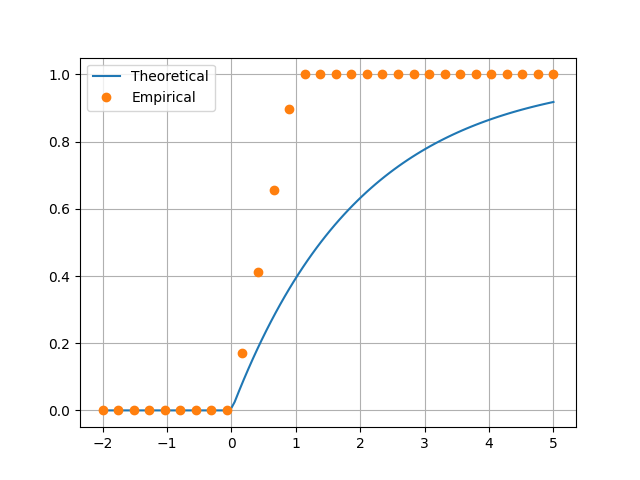
\includegraphics[width=\columnwidth]{figs/Figure_4.png}
		\caption{The CDF of $V$}
		\label{Figure_4}
	\end{figure}	
	
	\item Find a theoretical expression for $F_V(x)$
	
	\solution We have
	\begin{align}
		F_V(x) &= \pr{V \le x} \\
		&= \pr{-2\ln\brak{1-U} \le x} \\
		&= \pr{\ln\brak{1-U} \ge -\frac{x}{2}} \\
		&= \pr{1-U \ge \exp\brak{-\frac{x}{2}}} \\
		&= \pr{U \le 1 - \exp\brak{-\frac{x}{2}}} \\
		&= F_U\brak{1 - \exp\brak{-\frac{x}{2}}}
	\end{align}
	Now,
	\begin{align}
		0 \le 1-\exp\brak{-\frac{x}{2}} &< 1 \qquad \text{if } x \ge 0	\\	
		1-\exp\brak{-\frac{x}{2}} &< 0 \qquad \text{if } x < 0	
	\end{align}
	
	Therefore,
	\begin{align}
		F_V(x) = 
		\begin{cases}
			1-\exp\brak{-\dfrac{x}{2}} & x \ge 0 \\
			0 & x < 0
		\end{cases}
	\end{align}
	
	\end{enumerate}
	
\end{document}